% Sablon pentru realizarea lucrarii de licenta, conform cu recomandarile
% din ghidul de redactare:
% - https://fmi.unibuc.ro/finalizare-studii/
% - https://drive.google.com/file/d/1xj9kZZgTkcKMJkMLRuoYRgLQ1O8CX0mv/view

% Multumiri lui Gabriel Majeri, acest sablon a fost creat pe baza
% codului sursa a lucrarii sale de licenta. 
% Codul sursa: https://github.com/GabrielMajeri/bachelors-thesis
% Website: https://www.gabrielmajeri.ro/
%
% Aceast sablon este licentiat sub Creative Commons Attribution 4.0 International License.

\documentclass[12pt a4paper]{report}

%Enviroment nou pt a inlocui abstract din report
% \newenvironment{abstract}{
%     \chapter*{Abstract}
%     \addcontentsline{toc}{chapter}{Abstract}
%     \markboth{\MakeUppercase{Abstract}}{}
% }{
%     \clearpage
% }

\usepackage{times}

\usepackage{float}

% Suport pentru diacritice și alte simboluri
\usepackage{fontspec}

% Suport pentru mai multe limbi
\usepackage{polyglossia}

% Suport pentru enums
\usepackage{enumitem}

% Setează limba textului la română
\setdefaultlanguage{romanian}

% Am nevoie de engleză pentru rezumat
\setotherlanguages{english}

% Indentează și primul paragraf al fiecărei noi secțiuni
\SetLanguageKeys{romanian}{indentfirst=true}

% Font size
\fontsize{12}{14.4}\selectfont

% Suport pentru diferite stiluri de ghilimele
\usepackage{csquotes}

\DeclareQuoteStyle{romanian}
  {\quotedblbase}
  {\textquotedblright}
  {\guillemotleft}
  {\guillemotright}

% Utilizează biblatex pentru referințe bibliografice
\usepackage[
    maxbibnames=50,
    sorting=nty
]{biblatex}

\addbibresource{bibliography.bib}

% Setează spațiere inter-linie la 1.5
\usepackage{setspace}
\doublespacing

% Modificarea geometriei paginii
\usepackage{geometry}

% Include funcțiile de grafică
\usepackage{graphicx}
% Încarcă imaginile din directorul `images`
\graphicspath{{./images/}}

% Listări de cod
\usepackage{listings}

% Linkuri interactive în PDF
\usepackage[
    colorlinks,
    linkcolor={black},
    menucolor={black},
    citecolor={black},
    urlcolor={blue}
]{hyperref}

% Comenzi matematice
\usepackage{amsmath}
\usepackage{mathtools}

% Simboluri matematice codificate Unicode
\usepackage[warnings-off={mathtools-colon,mathtools-overbracket}]{unicode-math}

% Formule matematice
\newcommand{\bigO}[1]{\symcal{O}\left(#1\right)}
\DeclarePairedDelimiter\abs{\lvert}{\rvert}

% Suport pentru rezumat în două limbi
% Bazat pe https://tex.stackexchange.com/a/70818
\newenvironment{abstractpage}
  {\cleardoublepage\thispagestyle{empty}}
  {\vfill\cleardoublepage}
\renewenvironment{abstract}[1]
  {\cleardoublepage\bigskip\selectlanguage{#1}%
   \begin{center}\bfseries\abstractname\end{center}}
  {\par\bigskip}

% Suport pentru anexe
\usepackage{appendix}

% Stiluri diferite de headere și footere
\usepackage{fancyhdr}

% Mutam textul de la capitole putin mai la dreapta
\usepackage{tocloft}
\cftsetindents{chapter}{-0.5em}{2em} % primul e pt distanta cifrei fata de margine, a doua e pt distanta dintre cifra

% Metadate
\title{Proiectarea și implementarea arhitecturilor chatbot cu aplicații în industria bancară}
\author{Andriță Lucian-Gabriel}

% Generează variabilele cu @
\makeatletter

\begin{document}

% Front matter
\cleardoublepage
\let\ps@plain

% Coperta
\begin{titlepage}

% Redu marginile
\newgeometry{left=2cm,right=2cm,bottom=1cm}

\begin{figure}[!htb]
    \centering
    \begin{minipage}{0.2\textwidth}
        
\includegraphics[width=\linewidth]{logo-ub.png}
    \end{minipage}
    \begin{minipage}{0.5\textwidth}
        \large
        \vspace{0.2cm}
        \begin{center}
            \textbf{UNIVERSITATEA DIN BUCUREȘTI}
        \end{center}
        \vspace{0.3cm}
        \begin{center}
            \textbf{
                FACULTATEA DE \\
                MATEMATICĂ ȘI INFORMATICĂ
            }
        \end{center}
    \end{minipage}
    \begin{minipage}{0.2\textwidth}
        
\includegraphics[width=\linewidth]{logo-fmi.png}
    \end{minipage}
\end{figure}

\begin{center}
\textbf{SPECIALIZAREA TEHNOLOGIA INFORMAȚIEI}
\end{center}

\vspace{4cm}

\begin{center}
\huge \textbf{\MakeUppercase{Lucrare de licență}}
\end{center}

\vspace{3cm}

\begin{center}
\large \textbf{Absolvent \\ \@author}
\end{center}

\vspace{0.25cm}

\begin{center}
\large \textbf{Coordonator științific \\ Prof. dr. Cristian Kevorchian}
\end{center}

\vspace{2cm}

\begin{center}
\Large \textbf{București, iunie 2023}
\end{center}
\end{titlepage}

% Pagina de titlu
\begin{titlepage}

% Redu marginile
\newgeometry{left=2cm,right=2cm,bottom=1cm}

\begin{figure}[!htb]
    \centering
    \begin{minipage}{0.2\textwidth}
        
\includegraphics[width=\linewidth]{logo-ub.png}
    \end{minipage}
    \begin{minipage}{0.5\textwidth}
        \large
        \vspace{0.2cm}
        \begin{center}
            \textbf{UNIVERSITATEA DIN BUCUREȘTI}
        \end{center}
        \vspace{0.3cm}
        \begin{center}
            \textbf{
                FACULTATEA DE \\
                MATEMATICĂ ȘI INFORMATICĂ
            }
        \end{center}
    \end{minipage}
    \begin{minipage}{0.2\textwidth}
        
\includegraphics[width=\linewidth]{logo-fmi.png}
    \end{minipage}
\end{figure}

\begin{center}
\textbf{SPECIALIZAREA TEHNOLOGIA INFORMAȚIEI}
\end{center}

\vspace{1cm}

\begin{center}
\Large \textbf{Lucrare de licență}
\end{center}

\begin{center}
\huge \textbf{\MakeUppercase{\@title}}
\end{center}

\vspace{3cm}

\begin{center}
\large \textbf{Absolvent \\ \@author}
\end{center}

\vspace{0.25cm}

\begin{center}
\large \textbf{Coordonator științific \\ Prof. dr. Cristian Kevorchian}
\end{center}

\vspace{2cm}

\begin{center}
\Large \textbf{București, iunie 2023}
\end{center}
\end{titlepage}
\restoregeometry
\newgeometry{
    margin=2.5cm
}

\fancypagestyle{main}{
  \fancyhf{}
  \renewcommand\headrulewidth{0pt}
  \fancyhead[C]{}
  \fancyfoot[C]{\thepage}
}

% Rezumatul
\pagestyle{empty}
\begin{abstractpage}

\begin{abstract}{romanian}

Acesta este un șablon C++ care utilizează Dialogflow ES de la Google Cloud Platform pentru interacțiuni între oameni și chatbot în diferite contexte, în funcție de cazurile de utilizare ale întreținătorului. Această aplicație în particular folosește procesarea în cloud într-un context bancar și a fost creată ca o dovadă a unui concept, obiectivul principal fiind de a-mi extinde cunoștințele cu privire la interacțiunile C++ într-un mediu modern, utilizând diferite servicii cloud pentru a izola funcționalitățile principale ale aplicației, mutând implementarea locală într-una găzduită în cloud. 

Serverul care gestionează conexiunea între clienți și agent este găzduit local. Atunci când se primește o solicitare de la un client, serverul decide ce tip de fișiere să trimită. Pe măsură ce clientul își face interogari către agent, un script va acționa ca parser pentru textul dat și va asculta răspunsul de la server. Când serverul primește intrarea, o va trimite la agent. În cloud, agentul va potrivi textul primit cu o intenție, va extrage unii parametrii în funcție de intenție și va apela un webhook. Webhook-ul constă într-o funcție Google Cloud Function, care este găzduită pe Google Source Repository, unde va căuta în dosarul cloud și va extrage funcționalitatea de acolo. 

Funcția va avea privilegii CRUD+L asupra unui bucket Google Cloud Storage care stochează informațiile necesare. Acest studiu reprezintă o contribuție semnificativă la înțelegerea modului în care serviciile de cloud pot fi integrate cu succes în aplicațiile bazate pe C++, cu un accent specific pe dezvoltarea chatbot-urilor în industria bancară.
\end{abstract}

\begin{abstract}{english}

This is a C++ template that uses Google Cloud Platform's Dialogflow ES for human-chatbot interactions in different contexts, depending on the use cases of the maintainer. This particular application uses cloud processing in a banking context and was created as a proof of concept, its main goal being to further expand my knowledge regarding C++ interactions in a modern enviroment, while using different cloud services to isolate main functionalities of the application moving the local implementation to a cloud hosted one. 

The server that is serving the connection between the clients and the agent is locally hosted. When a request from a client is received, the server decides what type of files to send. As the client queries his intent to the agent, a script will act as a parser for the given text, and will listen for the response from the server. When the server receives the input, it will send it to the agent. In the cloud, the agent will match the received text with an intent, it will extract some parameters based on the intent, and it will call a webhook. The webhook consists of a Google Cloud Function, that's being hosted on Google Source Repository, where it will look into the cloud folder and extract the functionality from there. 

The function will have CRUD+L privileges on a Google Cloud Storage bucket that stores the needed information. This study represents a significant contribution to the understanding of how cloud services can be successfully integrated into C++ based applications, with a specific focus on the development of chatbots in the banking industry.
\end{abstract}

\end{abstractpage}

\addtocounter{page}{1}

% Modificare pentru cuprins
\pagestyle{empty}
\tableofcontents
\renewcommand{\thechapter}{\Roman{chapter}} % Chapter numbering: I, II, III, etc.
\renewcommand{\thesection}{\thechapter.\arabic{section}} % Section numbering: 1, 2, 3, etc.
\renewcommand{\thesubsection}{\thesection.\arabic{subsection}} % Subsection numbering: 1.1, 1.2, 2.1, 2.2, etc.
\renewcommand{\thesubsubsection}{\thesubsection.\arabic{subsubsection}} % Subsubsection numbering: 1.1.1, 1.1.2, 2.1.1, 2.1.2, etc.

% Main matter
\cleardoublepage
\pagestyle{main}
\let\ps@plain\ps@main

\chapter{Introducere}

\section{Nevoia migrării în cloud}

În era digitală modernă, tendința de procesare mutată în cloud a devenit o parte integrală a multor domenii și industrii. Această tendință se referă la transferul și executarea operațiunilor de procesare a datelor și sarcinilor complexe în cloud, în loc să fie realizate local.

Procesarea mutată în cloud oferă o abordare inovatoare și scalabilă pentru gestionarea volumelor mari de date și sarcini computaționale intensive. Prin intermediul infrastructurii cloud, această tendință permite accesul la resurse computaționale puternice și flexibile, oferind astfel utilizatorilor o experiență îmbunătățită și performanțe superioare în timp real \cite{benefits-of-cloud-computing}.

Prin transferarea sarcinilor în mediul cloud, utilizatorii beneficiază de o serie de avantaje. Unul dintre acestea este accesul la capacități de procesare și resurse de stocare extinse, care pot depăși de multe ori puterea de calcul a dispozitivelor individuale. Această scalabilitate permite utilizatorilor să gestioneze sarcini complexe, cum ar fi analiza unor seturi de date foarte mari, procesarea grafică avansată sau algoritmi de învățare automată, fără a se confrunta cu constrângerile tehnice ale dispozitivelor personale.

Pe lângă avantajele de performanță, procesarea mutată în cloud oferă și o mai mare flexibilitate și mobilitate. Utilizatorii pot accesa și gestiona datele și aplicațiile lor de pe diferite dispozitive, indiferent de locație sau de sistemul de operare utilizat. Acest aspect aduce un nivel crescut de colaborare și sincronizare între utilizatori, sporind eficiența și productivitatea în mediul de lucru modern.

Totuși, pe lângă beneficiile pe care le aduce, procesarea mutată în cloud aduce anumite provocări și preocupări. Una dintre ele este legată de securitatea datelor și confidențialitatea informațiilor. Deoarece datele sunt transferate și procesate în mediul cloud, există riscul ca acestea să fie expuse la amenințări cibernetice sau să fie accesate de persoane neautorizate. Drept urmare, furnizorii de servicii cloud trebuie să implementeze măsuri solide de securitate și criptare pentru a proteja datele utilizatorilor.

\section{Scopul lucrării}

Aplicația este un template care îmbină procese moderne de prelucrare și stocare a datelor folosind servicii cloud. Scopul acesteia este de a fi o implementare practică a unui concept și de a-mi îmbunătăți cunoștiințele cu privire la servicii cloud, arhitectură de aplicații, limbajul C++, clean coding, precum și best practices în acest context. Codul sursă se poate găsi pe pagina personală de GitHub \cite{github}.

Alegerea unui limbaj precum C++ pentru dezvoltarea unei aplicații web a prezentat o provocare în ceea ce privește alegerea utilitarului potrivit pentru crearea și gestionarea serverului. Multe aplicații întâlnite folosesc JavaScript și utilitare pentru conectarea la diferiți furnizori de servicii cloud, astfel curiozitatea mea m-a făcut să mă întreb de aplicabilitatea unor alte suite de tehnologii pentru o astfel de aplicație, păstrând totuși ideea centrală de utilizare a cât mai multe servicii cloud pentru diferite functionalități.

\section{Obiective}

În partea de implementare propriu-zisă, am avut în vedere câteva obiective:

\begin{enumerate}
    \item Investigarea caracteristicilor unice ale Dialogflow și motivul pentru care acesta este o alegere potrivită pentru dezvoltarea chatbotilor în sisteme bancare.
    \item Proiectarea și implementarea unui model de chatbot bazat pe Dialogflow, specializat pentru utilizare în sistemul bancar. Acesta ar trebui să fie capabil să răspundă la întrebări frecvente, să ajute clienții să-și gestioneze conturile și tranzacțiile.
    \item Evaluarea performanței modelului de chatbot, în ceea ce privește acuratețea și promptitudinea răspunsurilor, precum și satisfacția generală a utilizatorilor.
    \item Explorarea viitoarelor posibilități de îmbunătățire și adaptare a chatbotilor pentru a răspunde mai bine nevoilor utilizatorilor de servicii bancare.
\end{enumerate}

\section{Contribuția personală}

În cadrul acestei lucrări de diplomă, am adus o contribuție personală semnificativă prin dezvoltarea și implementarea unui sistem de gestionare bancar care utilizează limbajul de programare C++. Alegerea utilizării limbajului C++ în detrimentul altor limbaje mai frecvent utilizate în acest context a reprezentat o abordare inovatoare și a adus multiple beneficii proiectului.

Una dintre contribuțiile mele esențiale constă în adaptarea limbajului C++ pentru a se potrivi nevoilor specifice ale sistemului de gestionare a conversațiilor. De asemenea, am utilizat biblioteci și framework-uri specializate pentru a facilita interacțiunea cu serviciul Dialogflow și pentru a asigura o funcționalitate completă și robustă a sistemului.

Prin utilizarea limbajului C++, am demonstrat că acesta poate fi o opțiune viabilă și performantă în dezvoltarea sistemelor de gestionare a conversațiilor, în ciuda faptului că alte limbaje, precum JavaScript, sunt mai des întâlnite în acest domeniu. Am demonstrat abilitățile mele de programare în C++, precum și capacitatea de a înțelege și implementa tehnologii complexe, adaptându-le în mod eficient pentru a îndeplini cerințele proiectului.

\section{Motivația personală}

Într-o eră în care tehnologia se dezvoltă cu o rapiditate neegalată, am ales să îmi concentrez lucrarea de licență asupra unui subiect care mă fascinează: arhitectura de tip chatbot în sisteme bancare. Această alegere nu a fost aleatorie, ci a fost alimentată de interesul meu pentru dezvoltarea software, în special în limbajul C++, și de dorința de a explora potențialul aplicațiilor cloud în acest domeniu.

Încă de la începutul studiilor mele, am fost atras de complexitatea și puterea limbajului de programare C++. Acest limbaj mi-a oferit posibilitatea de a construi soluții software robuste, eficiente și flexibile. Dezvoltarea mea personală în acest sens a reprezentat o provocare continuă, dar și o sursă constantă de satisfacție. Alegerea acestei teme pentru lucrarea mea de licență este o oportunitate excelentă de a îmbina abilitățile mele în programarea C++ cu cele în AI și cloud computing.

În ultimii ani, am urmărit cu interes cum organizațiile bancare au început să adopte soluții bazate pe AI pentru a îmbunătăți serviciile pentru clienți și pentru a eficientiza operațiunile interne. Deși există multe implementări de succes (de exemplu ADA \cite{ADA}, asistentul virtual BCR), acest domeniu încă prezintă un potențial incomplet exploatat. Existența acestui potențial mi-a stârnit curiozitatea și m-a determinat să încerc să răspund la următoarea întrebare: este cu adevărat realizabil un sistem de chatbot eficient și complet bazat pe text, fără alt tip de input?

În plus, sunt convins că utilizarea tehnologiei cloud în dezvoltarea acestui chatbot nu va îmbunătăți doar scalabilitatea și disponibilitatea sistemului, dar va permite și implementarea mai ușoară a unor funcționalități avansate de AI. Prin utilizarea serviciului Dialogflow, mă aștept să pot dezvolta un chatbot capabil să îmbunătățească în mod semnificativ interacțiunea dintre bănci și clienții lor.

Așadar, am ales această temă de licență deoarece îmi oferă oportunitatea de a explora aceste idei în detaliu și de a contribui la dezvoltarea soluțiilor tehnologice în domeniul bancar, dar și pentru a-mi deschide și alte porți cu privire la înțelegerea legăturilor dintre servicii cloud independente.

\section{Scurt istoric al integrării asistenților virtuali}

Introducerea asistenților virtuali în sistemele bancare din România a reprezentat un pas semnificativ în modernizarea și digitalizarea serviciilor financiare. Cu o populație tot mai conectată la tehnologie și cu un sector financiar dinamic și inovator, România se aliniază la tendințele globale, îmbrățișând avantajele oferite de inteligența artificială și de tehnologia cloud.

Primii pași în această direcție s-au făcut în ultimii ani, mai exact în 2017, când băncile românești au început să recunoască nevoia de a oferi servicii mai eficiente și mai personalizate clienților lor. Prima bancă românească care a introdus un asistent virtual a fost Banca Transilvania, ea lansând chatbot-ul \emph{Livia} \cite{first-chatbot}. Confruntate cu o concurență acerbă și cu așteptările tot mai mari ale clienților, instituțiile bancare au început să exploreze diferite soluții tehnologice. 

În acest context, asistenții virtuali au apărut ca un instrument promițător pentru îmbunătățirea experienței clientului. Următorul pas pentru Banca Transilvania a fost să migreze în 2019 către platforma Druid, platformă ce se ocupă de dezvoltarea chatbotilor conversaționali. Aceasta tendință a fost urmată și de către BCR, ADA fiind construită tot pe Druid \cite{ADA}.

Asistenții virtuali în serviciile bancare au rolul de a fluidiza interacțiunile cu clienții și de a îmbunătăți calitatea serviciilor. Ei pot răspunde în timp real la o gamă largă de întrebări, pot efectua tranzacții simple în numele clienților și pot oferi asistență personalizată, reducând astfel timpul de așteptare și îmbunătățind satisfacția clientului.

Implementarea asistenților virtuali nu a fost fără provocări. Pe lângă dificultățile tehnice, a fost necesară depășirea reticenței unor clienți de a schimba modul în care interacționau cu orice serviciu bancar, fiind în natura umană de a încerca să nu ieși din zona ta de comfort. În plus, au fost necesare eforturi considerabile pentru a asigura securitatea datelor și pentru a respecta reglementările privind confidențialitatea.

Cu toate acestea, beneficiile pe care le aduc chatbotii în sistemul bancar sunt semnificative. În primul rând, ei pot funcționa non-stop, asigurând asistență clienților în orice moment al zilei sau al nopții. În al doilea rând, pot gestiona un volum mare de solicitări simultan, ceea ce este dificil de realizat pentru angajații umani. În al treilea rând, folosirea chatbotilor poate reduce costurile operaționale, întrucât necesită mai puține resurse umane.

Deși este încă la început, implementarea asistenților virtuali în sistemele bancare din România arată promițător. Cu un nivel din ce în ce mai mare de acceptare și cu progresele continue în tehnologia AI, chatbotii vor ajunge să joace un rol tot mai important în transformarea digitală a sectorului bancar românesc și nu numai.

\section{Structura lucrării}

Lucrarea este structurată în următoarele capitole:

\begin{enumerate}
    \item \textbf{Introducere}: prezintă o viziune generală asupra conținutului lucrării, punând accent pe tendința modernă de mutare a procesării în cloud cât și automatizarea proceselor prin chatboti conversaționali.
    \item \textbf{Preliminarii}: explică elementele cheie ale lucrării și subdomeniului de care aceasta aparține.
    \item \textbf{Decizii arhitecturale}: descrie modul de funcționare al platformei alese (Google Cloud Platform) cât și beneficiile utilitarului POCO față de alte librării.
    \item \textbf{Setup și compilare}: explică procesul de configurare și compilare al aplicației.
    \item \textbf{Detalierea implementării}: explică design-ul cât și funcționalitatea aplicației.
    \item \textbf{Concluzii}: această secțiune sintetizează informațiile discutate și propune posibile direcții de dezvoltare pentru viitor.
\end{enumerate}
\chapter{Preliminarii}

\section{Noțiuni de bază}

Înainte de a ne aprofunda în analiza specifică a acestei lucrări, este important să înțelegem câteva noțiuni fundamentale care stau la baza dezvoltării și implementării unui asistent virtual în domeniul bancar.

\begin{itemize}
    \item \textbf{Chatbot} 

Chatbotul este un program software ce simulează o conversație umană. În mod tradițional, utilizatorii interacționează cu chatbotii prin intermediul unei interfețe textuale, deși unii chatboti moderne pot interacționa și prin comenzi vocale.

Există două tipuri principale de chatboti: chatbotii bazati pe reguli și chatbotii bazati pe învățarea automată. Chatbotii bazati pe reguli sunt proiectați pentru a răspunde la întrebări specifice și sunt programați cu un set de reguli predefinite. Pe de altă parte, chatbotii bazati pe învățare automată se bazează pe algoritmi de inteligență artificială și sunt capabili să învețe din interacțiunile cu utilizatorii.

În industria bancară, chatbotii sunt utilizati în special în serviciul de asistență pentru clienți, unde pot răspunde la întrebări frecvente, pot ajuta la rezolvarea problemelor și pot ghida utilizatorii prin diferite procese.

    \item \textbf{Tehnologia Cloud}

Tehnologia cloud se referă la livrarea de servicii IT prin internet, în loc de a folosi infrastructura fizică locală. Aceasta poate include servicii de calcul, stocare, baze de date, rețelistică, software, analize și inteligență.

Există trei tipuri principale de servicii cloud: Infrastructură ca Serviciu (IaaS), Platformă ca Serviciu (PaaS) și Software ca Serviciu (SaaS). În industria bancară, cloud computing-ul poate ajuta la reducerea costurilor, la îmbunătățirea eficienței operaționale și la scalabilitate.

    \item \textbf{Inteligenta artificială} 

Inteligența Artificială (AI) se referă la simularea inteligenței umane de către mașini, în special sistemele informatice. Sarcinile AI pot include învățarea (abilitatea de a dobândi și aplica cunoștințe și abilități), raționamentul (utilizarea de reguli pentru a ajunge la concluzii aproximative sau definite), auto-corectarea și procesarea limbajului natural.

Chatbotii bazati pe AI, cum ar fi cei dezvoltati cu DialogFlow, pot învăța din interacțiuni și pot îmbunătăți continuu calitatea conversațiilor pe care le au cu utilizatorii.

    \item \textbf{DialogFlow}

DialogFlow, deținut de Google, este o platformă care permite dezvoltatorilor să creeze interfețe de conversație pentru site-uri web, aplicații mobile și platforme populare de mesagerie \cite{sharma2018}. DialogFlow utilizează tehnologia de înțelegere a limbajului natural (NLU - \emph{Natural Language Understanding}) pentru a înțelege și a procesa limbajul uman.

În contextul dezvoltării chatbotilor pentru instituțiile bancare, DialogFlow poate ajuta la crearea de boti care să înțeleagă și să răspundă la cererile utilizatorilor într-un mod mai natural și mai intuitiv.

\end{itemize}

\section{Stadiul actual al subdomeniului}

Implementarea chatbotilor în sistemul bancar reprezintă o inovație semnificativă în modul în care băncile interacționează cu clienții lor. Începând cu Banca Transilvania în 2017, multe alte instituții bancare din România au urmat exemplul și au început să folosească chatboti pentru a îmbunătăți serviciile oferite clienților.

Chatbotii oferă un nivel de disponibilitate non-stop, care este deosebit de valoros într-o industrie precum cea bancară, care necesită suport pentru clienți la orice oră. Prin eliminarea nevoii de interacțiune umană pentru a rezolva probleme comune, chatbotii permit băncilor să economisească resurse și să se concentreze pe probleme mai complexe. Acești asistenți virtuali pot răspunde rapid la întrebări, pot rezolva probleme și pot oferi asistență în tranzacții financiare, îmbunătățind astfel satisfacția generală a clienților.

Cu toate acestea, în ciuda progreselor semnificative în adoptarea tehnologiei chatbot în industria bancară, există încă multe oportunități de explorare și îmbunătățire. Un domeniu cheie de cercetare este îmbunătățirea înțelegerii naturale a limbajului de către chatboti. Deși chatbotii actuali sunt capabili să gestioneze o serie de interacțiuni de bază, abilitatea lor de a înțelege nuanțele și complexitatea limbajului uman este limitată.

Un alt domeniu de potențială îmbunătățire este personalizarea și adaptabilitatea. În prezent, majoritatea chatbotilor bancari folosesc algoritmi pre-programați pentru a răspunde la interacțiunile utilizatorilor. Cu toate acestea, există oportunități semnificative pentru utilizarea tehnologiilor avansate de AI, cum ar fi învățarea profundă, pentru a dezvolta chatboti care pot învăța și se pot adapta la comportamentul și preferințele individuale ale utilizatorilor.

\begin{figure}[h] % h = here, adica pune figura fix unde e textul
    \centering
    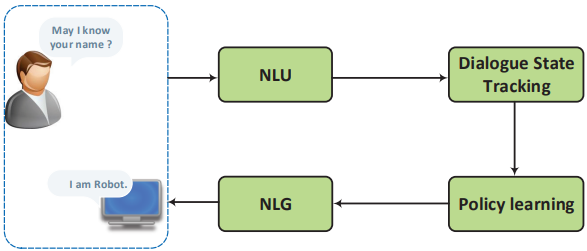
\includegraphics[scale=0.7]{traditional-pipeline}
    \caption{Pipeline general pentru sisteme orientate pe task-uri \cite{chen_liu_yin_tang_dialogue_2017}}
\end{figure}

În plus, există încă multe provocări legate de securitate și confidențialitate care trebuie abordate înainte ca chatbotii să fie adoptați pe scară largă în industria bancară. Acestea includ protejarea datelor personale și financiare ale utilizatorilor și asigurarea că chatbotii nu pot fi utilizați pentru activități frauduloase.

În concluzie, în timp ce adoptarea chatbotilor în sistemul bancar a făcut progrese remarcabile în ultimii ani, există încă multe oportunități de cercetare și dezvoltare în acest domeniu. Pe măsură ce tehnologia continuă să avanseze, este de așteptat ca chatbotii să devină un element tot mai integral al serviciilor bancare.

\section{Obiectivele lucrării în context}

Obiectivul principal al acestei lucrări este de a investiga posibilitățile pe care tehnologia chatbot și serviciile cloud le oferă în contextul sistemului bancar. În particular, accentul este pus pe implementarea unui model de chatbot bazat pe platforma DialogFlow, cu suport pentru limbajul de programare C++. C++ este un limbaj de programare popular, cunoscut pentru eficiența și puterea sa, fiind astfel un candidat potrivit pentru dezvoltarea unui chatbot robust și eficient.

În actualul stadiu de dezvoltare a tehnologiei chatbot, această lucrare vizează să contribuie la progresul subdomeniului, prin oferirea unei viziuni detaliate asupra procesului de implementare a unui chatbot în serviciile bancare, lucrarea speră să aducă o valoare semnificativă domeniului.

În plus, lucrarea explorează și potențialele căi de îmbunătățire și adaptare a chatbotilor. O astfel de direcție ar putea fi folosirea de tehnologii avansate de AI, cum ar fi învățarea profundă, pentru a dezvolta chatboti care pot învăța și se pot adapta la comportamentul și preferințele individuale ale utilizatorilor. Prin urmare, acest studiu își propune să deschidă calea către o utilizare mai extinsă și mai eficientă a tehnologiei chatbot în industria bancară.

Pe de altă parte, această lucrare se concentrează și asupra cloud computing-ului, o tehnologie care a revoluționat modul în care datele și serviciile sunt gestionate. Cu ajutorul cloud computing-ului, chatbotii pot fi ușor scalabili, ceea ce înseamnă că pot servi un număr mare de utilizatori simultan, fără a compromite performanța. În plus, cloud computing-ul facilitează actualizările și îmbunătățirile continuu, fără întreruperi majore ale serviciului \cite{mell_grance2011}.

În concluzie, această lucrare are ca scop principal să demonstreze cum tehnologiile moderne, precum chatbotii și cloud computing-ul, pot transforma modul în care băncile interacționează cu clienții lor. Se urmărește evidențierea beneficiilor potențiale ale utilizării agenților conversaționali pentru optimizarea proceselor și serviciilor bancare, în speranța de a stimula o adoptare mai largă a acestor tehnologii în industria bancară.
\chapter{Ecosistemul Google Cloud}

\section{Alegerea platformei agentului}

Comparând Dialogflow cu alte servicii de agenți conversaționali, există mai multe caracteristici care o diferențiază și recomandă pentru utilizarea în sectorul bancar.

Dialogflow, deținut de Google, este o platformă avansată pentru dezvoltarea de aplicații de conversație, care folosește tehnologia AI pentru a interpreta intențiile și contextul utilizatorului \cite{google_dialogflow}. Aceasta oferă o gamă largă de funcționalități, inclusiv integrarea cu diverse platforme de mesagerie, asistenți virtuali și alte servicii Google, cum ar fi Google Cloud Functions.

La rândul lor, serviciile alternative, cum ar fi IBM Watson, Amazon Lex și Microsoft Luis, prezintă și ele avantaje. IBM Watson se remarcă prin puterea sa de a învăța în mod continuu și de a se adapta la diverse contexte de utilizare \cite{ibm_watson}. Amazon Lex beneficiază de integrarea nativă cu ecosistemul Amazon Web Services (AWS), oferind posibilități extinse de dezvoltare și scalare \cite{amazon_lex}. Între timp, Microsoft Luis are avantajul integrării strânse cu suita de produse Microsoft, incluzând Office 365 și Azure \cite{microsoft_luis}.

Cu toate acestea, Dialogflow se distinge prin mai multe aspecte-cheie. În primul rând, Dialogflow este foarte flexibil, permițând dezvoltatorilor să creeze experiențe de conversație personalizate pentru diferite platforme și canale de comunicare. Acesta poate fi integrat cu o multitudine de servicii, de la Google Assistant și Amazon Alexa, până la Facebook Messenger și Slack.

În al doilea rând, Dialogflow este strâns integrat cu ecosistemul Google Cloud. Acesta permite dezvoltatorilor să creeze, să testeze și să implementeze chatboti direct în cloud, profitând de avantajele cloud computing, inclusiv scalabilitatea, redundanța și accesul la cele mai recente inovații AI.

Aici intervine Google Cloud Functions \cite{google_cloud_functions}, un serviciu de calcul care permite dezvoltatorilor să execute cod ca răspuns la evenimente specifice, fără a fi nevoie să administreze o infrastructură de server. Acest serviciu poate fi utilizat în tandem cu Dialogflow pentru a crea funcții de backend pentru chatbot, cum ar fi procesarea cererilor utilizatorului, integrarea cu alte sisteme sau baze de date, sau gestionarea autentificării și a securității.

Google Cloud Functions se integrează perfect cu Google Source Repositories \cite{google_source_repositories}, un serviciu de găzduire de cod sursă care oferă un loc sigur și scalabil pentru a stoca și a gestiona codul. Acest lucru permite dezvoltatorilor să colaboreze eficient la proiecte, să gestioneze versiunile de cod și să implementeze automat codul în Cloud Functions.

În final, Google Cloud Storage oferă un serviciu de stocare de obiecte scalabil și durabil, care poate fi utilizat pentru a stoca și a servi datele utilizate de chatbot, cum ar fi înregistrări de conversații, profile de utilizator, sau alte date de context \cite{google_cloud_storage}.

\begin{figure}[h]
    \centering
    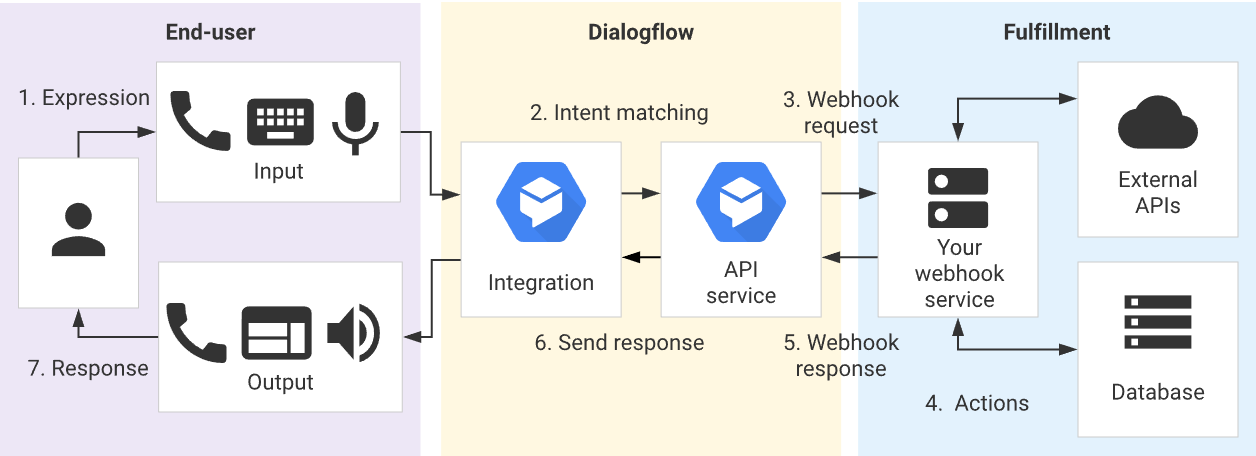
\includegraphics[scale=0.4]{fulfillment-flow}
    \caption{Flow-ul intern al Dialogflow \cite{google_dialogflow}}
\end{figure}

În ansamblu, alegerea Dialogflow, împreună cu Google Cloud Functions, Google Source Repositories și Google Cloud Storage, oferă o soluție robustă și flexibilă pentru dezvoltarea de chatboti în sectorul bancar. Prin folosirea acestor tehnologii, băncile pot crea experiențe de conversație personalizate, eficiente și securizate pentru clienții lor.

\section{Cum funcționează ecosistemul?}

Dialogflow folosește input-ul trimis de către Dialogflow API C++ Client \cite{dialogflow_client_library}, acesta fiind parsat și este trecut prin verificarea lor internă cu intențiile create în prealabil\footnote{O intenție reprezintă un anumit rezultat pe care doriți să îl obțineți de la interacțiunea utilizatorului. De exemplu, o intenție poate fi „programare întâlnire” sau „informații despre cont”.}. În funcție de cum este creat intent-ul și scopul său, pot exista parametrii scoși sub formă de entități\footnote{Entitățile sunt concepte valoroase care pot fi extrase din declarațiile utilizatorilor. De exemplu, în declarația „Doresc să programez o întâlnire pentru marți”, „marți” este o entitate de tip „dată”. Entitățile pot fi create în secțiunea „Entități” și pot fi asociate cu anumite intenții.} din textul primit (sau este un intent default, cu rol de legătură între altele cu functionalități).

\begin{figure}[h]
    \centering
    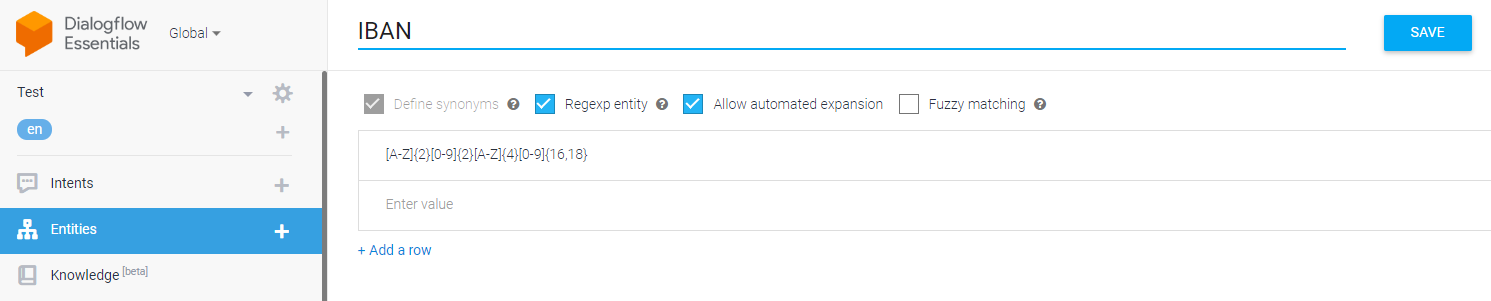
\includegraphics[scale=0.4]{entitati}
    \caption{Reprezentarea unei entități pentru IBAN folosind un regex}
\end{figure}

În cadrul platformei există niște entități predefinite \cite{system-entities} pentru a ușura munca utilizatorului atunci când vine vorba de extragere de parametrii
\chapter{Implementare}

\chapter{Concluzii}

\begin{appendix}
\chapter{Request-ul trimis către webhook}

\label{annex:request}

\begin{figure}[h]
    \centering
    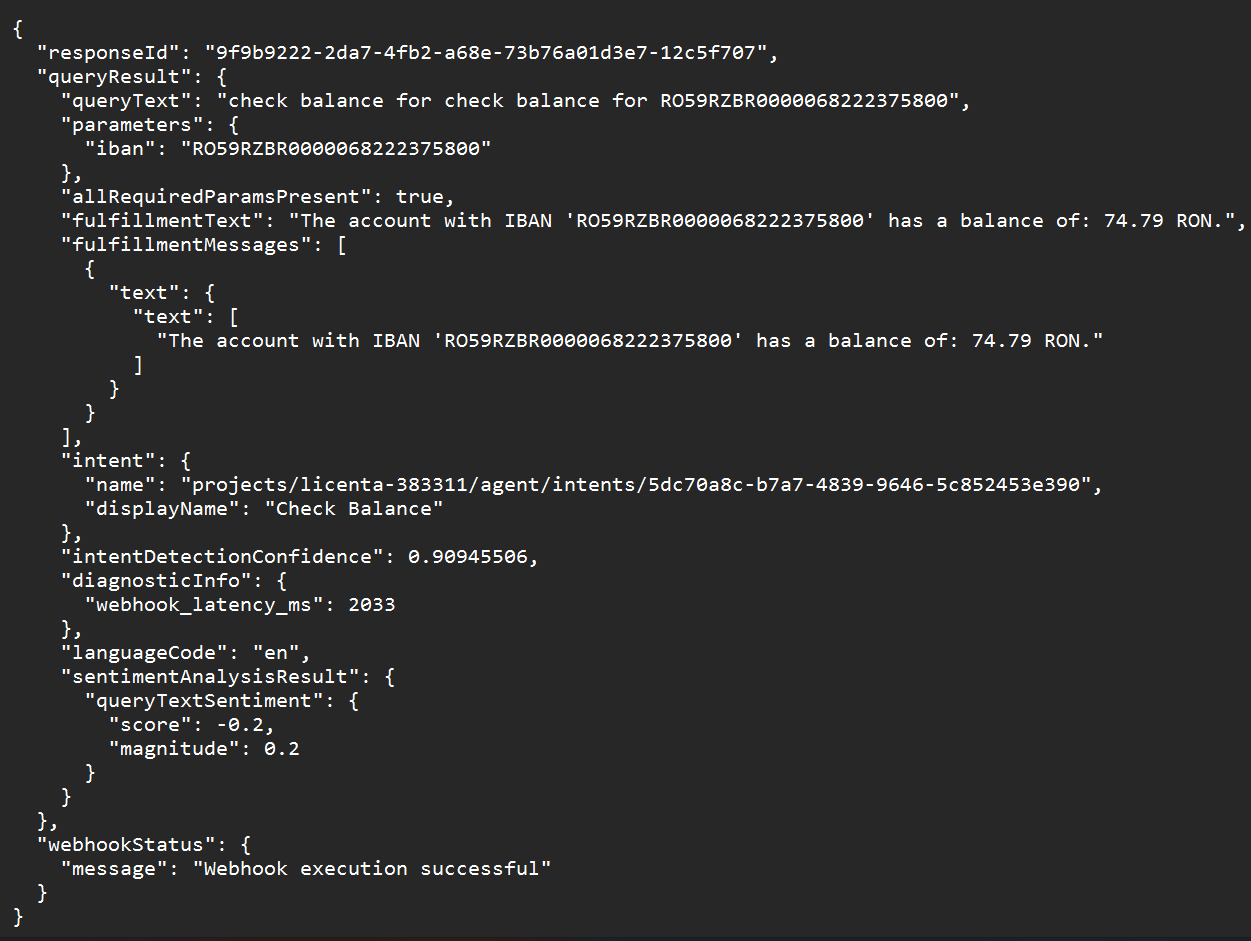
\includegraphics[width=1.0\textwidth]{exemplu-request}
    \caption{Exemplu de request trimis către Google Cloud Function}
    \label{fig:exemplu-request}
\end{figure}

\cleardoublepage

\begin{enumerate}
    \item responseId: acesta este un identificator unic pentru fiecare interacțiune cu DialogFlow.

    \item queryResult: aceasta este secțiunea care conține majoritatea informațiilor legate de interacțiunea cu utilizatorul.
    
    \subitem queryText: aceasta este întrebarea sau afirmația pe care utilizatorul a transmis-o.
    
    \subitem parameters: acestea sunt parametrii extrasi din întrebarea utilizatorului. În acest caz, "iban" este un parametru și valoarea sa este "RO59RZBR0000068222375800".
    
    \subitem allRequiredParamsPresent: acest câmp indică dacă toți parametrii necesari pentru intenție sunt prezenți. În acest caz, este adevărat, ceea ce înseamnă că toți parametrii necesari sunt prezenți.
    
    \subitem fulfillmentText: acesta este textul care va fi returnat utilizatorului ca răspuns la întrebarea sa.
    
    \subitem fulfillmentMessages: aceasta este o listă de mesaje care vor fi trimise înapoi utilizatorului. În acest caz, este doar un mesaj, care este același cu fulfillmentText.
    
    \subitem intent: aceasta este intenția care a fost potrivită pentru întrebarea utilizatorului.
    
    \subitem intentDetectionConfidence: acesta este gradul de încredere cu care DialogFlow a potrivit intenția. În acest caz, este de aproximativ 93%.
    
    \subitem diagnosticInfo: acestea sunt informații suplimentare privind interacțiunea. În acest caz, indică timpul de latență pentru webhook.
    
    \subitem languageCode: acesta este codul de limbă al interogării utilizatorului.
    
    \subitem sentimentAnalysisResult: aceasta este analiza sentimentului textului interogării. Scorul indică sentimentul general (pozitiv sau negativ), iar magnitudinea indică intensitatea sentimentului.
    
    \item webhookStatus: acesta este statusul execuției webhook-ului, care în acest caz a fost reușită.
\end{enumerate}
\chapter{Exemplu conversație}

\label{annex:exempluConversatie}

\begin{figure}[h]
    \centering
    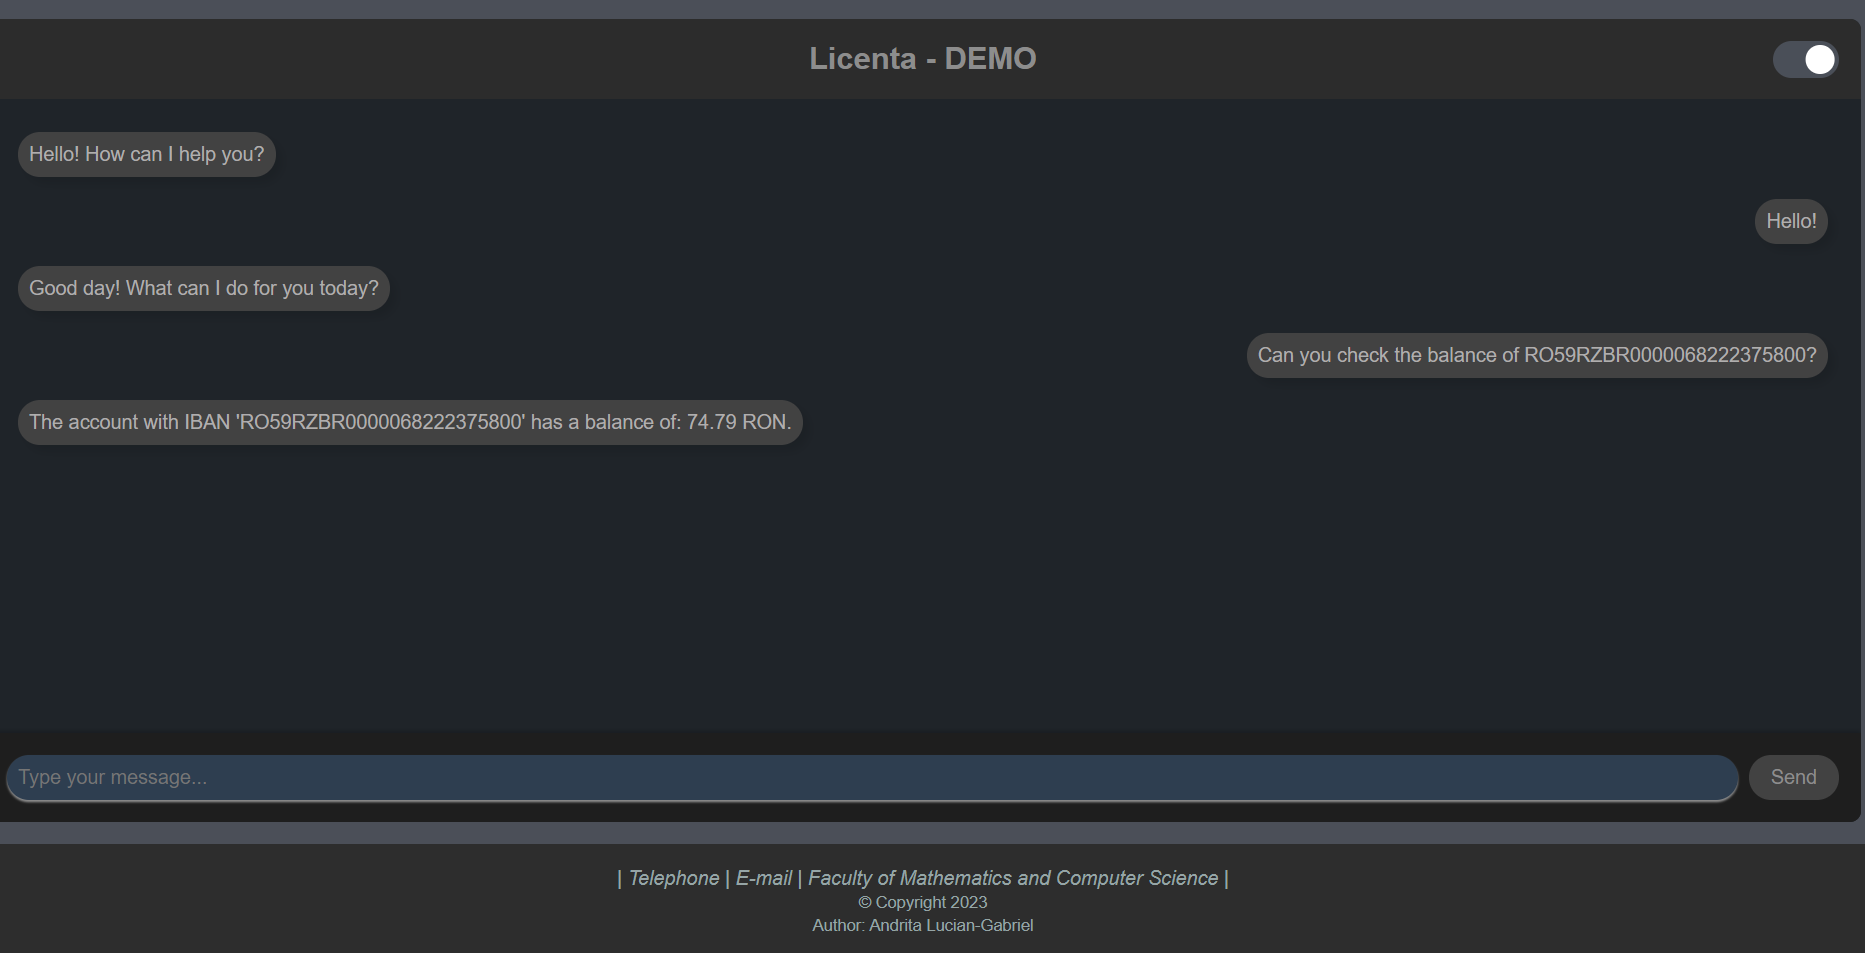
\includegraphics[width=1.0\textwidth]{exemplu-conversatie}
    \caption{Exemplu conversație}
    \label{fig:exemplu-request}
\end{figure}
\end{appendix}

\printbibliography[heading=bibintoc]

\end{document}